\section{Visualization I}
Some people look at a \svdl \ and see a hopeless jumble of numbers. But if we look at the decomposition in a different light, we can see alluring patterns and regularity. Our brains are better suited to remember these patterns than to remember formulation. This chapter dispenses with formal mathematics and captures interest by displaying the decompositions from a different perspective.

Let's pick a few simple matrices and look at a representation of their \svdl s.

%%%%
\subsection{Fundamental matrix types}
We will look at several different matrix types. Some are rank one, some are low rank, others full rank. This will produce a spectrum of decomposition products. Here are the type of matrices we will look at:
\begin{enumerate}
\item cross,
\item diamond,
\item disk,
\item Gaussian,
\item Hilbert,
\item Hankel,
\item Toeplitz,
\item ramp,
\item random,
\item tones I,
\item tones II,
\item trigonometric.
\end{enumerate}

For example, let's take the Hilbert matrix, the archetypical ill-conditioned matrix. The matrix element in row $r$, column $c$ is given as this:
\begin{equation}
  a_{rc} = \recip{r+c-1}.
  \label{eq:8:Hilbert}
\end{equation}
A sample matrix from this class is given here:
\begin{equation}
  \A{} = 
  \mat{cccccccc}{
           1 & \frac{1}{2} & \frac{1}{3} & \frac{1}{4} & \frac{1}{5} \\
 \frac{1}{2} & \frac{1}{3} & \frac{1}{4} & \frac{1}{5} & \frac{1}{6} \\
 \frac{1}{3} & \frac{1}{4} & \frac{1}{5} & \frac{1}{6} & \frac{1}{7} \\
 \frac{1}{4} & \frac{1}{5} & \frac{1}{6} & \frac{1}{7} & \frac{1}{8} \\
 \frac{1}{5} & \frac{1}{6} & \frac{1}{7} & \frac{1}{8} & \frac{1}{9} \\
}
\end{equation}
We can visualize this matrix by looking at the magnitude of each entry in gray scale. The element with the largest magnitude is solid black, zero entries are white.
\begin{table*}[htdp]
\begin{center}
\begin{tabular}{m{0.5in}m{1.25in}}
    $\A{} =$ &
    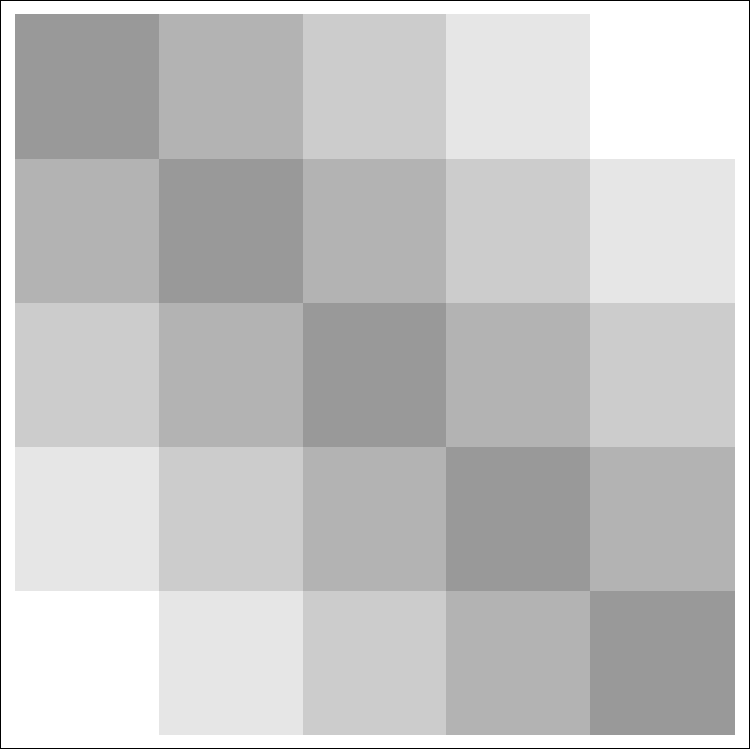
\includegraphics[ width = 1.5in ]{pdf/"ch 09"/"Hilbert"/A__0005}
\end{tabular}
\end{center}
%\label{default}
%\caption{default}
\end{table*}%
We will follow a convention where 1 is white and 0 is black. In between, there is gray. The decomposition looks like this:

\begin{table*}[htdp]
\begin{center}
\begin{tabular}{m{0.5in}m{1.25in}m{1.25in}m{1.25in}}
    $\svd{T} =$ &
    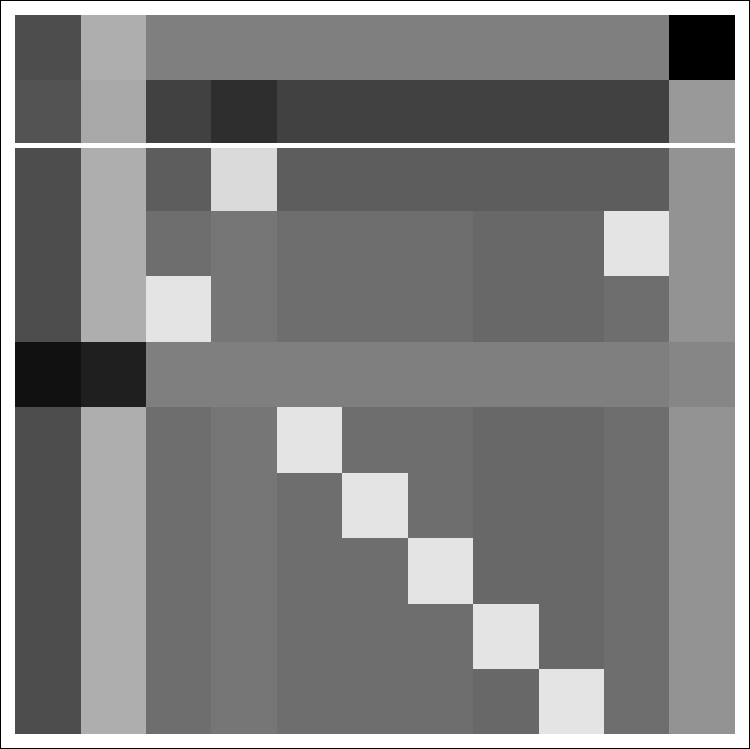
\includegraphics[ width = 1.25in ]{pdf/"ch 09"/"Hilbert"/Y__0005} &
    
\includegraphics[ width = 1.25in ]{pdf/"ch 09"/"Hilbert"/S__0005} &
    
\includegraphics[ width = 1.25in ]{pdf/"ch 09"/"Hilbert"/Xt_0005}
\end{tabular}
\end{center}
%\label{default}
%\caption{default}
\end{table*}%


Most of the matrix classes correspond to a specific definition in \emph{Mathematica}. Formal definitions follow. 
%%%%
\subsubsection{Cross matrix}
The cross matrix is a basic convolution filter. When $n=2$ the matrix has the form
\begin{equation}
  \A{} = 
  \mat{ccccc}{
 0 & 0 & 1 & 0 & 0 \\
 0 & 0 & 1 & 0 & 0 \\
 1 & 1 & 1 & 1 & 1 \\
 0 & 0 & 1 & 0 & 0 \\
 0 & 0 & 1 & 0 & 0
}.
\end{equation}
This matrix has two independent rows so the rank is $\rho = 2$.
%%%%
\subsubsection{Diamond matrix}
The diamond matrix is a another convolution filter. When $n=2$ the matrix has the form
\begin{equation}
  \A{} = 
  \mat{ccccc}{
 0 & 0 & 1 & 0 & 0 \\
 0 & 1 & 1 & 1 & 0 \\
 1 & 1 & 1 & 1 & 1 \\
 0 & 1 & 1 & 1 & 0 \\
 0 & 0 & 1 & 0 & 0
}.
\end{equation}
When the matrix has dimensions $\byy{2n+1}$ it will have rank $n+1$.

%%%%
\subsubsection{Disk matrix}
The disk matrix is the final convolution filter. When $n=2$ the matrix has the form
\begin{equation}
  \A{} = 
  \mat{ccccc}{
 0 & 1 & 1 & 1 & 0 \\
 0 & 1 & 1 & 1 & 0 \\
 1 & 1 & 1 & 1 & 1 \\
 0 & 1 & 1 & 1 & 0 \\
 0 & 1 & 1 & 1 & 0
}.
\end{equation}
The rank is not a smooth function of $n$ as seen in figure \eqref{fig:8:diskrank}. A rule of thumb is that the rank will be $0.6n$.
\begin{figure}[htbp] %  figure placement: here, top, bottom, or page
   \centering
   \includegraphics[ ]{pdf/"ch 08"/"08 disk rank"} 
   \caption[The rank of the disk matrix]{The rank of the disk matrix. A good rule of thumb is that the rank is  $\rho \approx 0.6n$.}
   \label{fig:8:diskrank}
\end{figure}%%%%

\subsubsection{Gaussian matrix}
This is a rank one matrix based upon the function
\begin{equation}
  f(x,y) = e^{-x^{2}} e^{-y^{2}}
\end{equation}
over the domain $D = \brac{0,1} \times \brac{0,1}$. As the matrix size increases the mesh is becoming finer. The matrix is rank one because each row is a multiple of the function
\begin{equation}
  g(x) = e^{x^{2}}.
\end{equation}
In fact this multiple is based upon the function
\begin{equation}
  g(y) = e^{y^{2}}.
\end{equation}
This reveals that the function can be expressed in separated form:
\begin{equation*}
  f(x,y) = g(x)g(y).
\end{equation*}
This separated form clarifies why the matrix will have rank one. A row corresponds to $y=$constant. This means that $x\in\brac{0,1}$ is multiplied by a number.
\begin{figure}[htbp] %  figure placement: here, top, bottom, or page
   \centering
   \includegraphics[ ]{pdf/"ch 08"/gaussian/"gaussian rows"} 
   \caption[Anatomy of a rank one matrix]{Anatomy of a rank one matrix. This is the plot the 21 elements in each of the first five rows of the Gaussian matrix. The rows are labelled. Every row is a multiple of every other row. The points represent the values of the matrix elements; the lines are added to make the plot readable.}
   \label{fig:pictures:gaussian:rankone}
\end{figure}
We will quickly look at powers of the Gaussian; we will soften and sharpen the peak. Even though we will still be dealing with rank one matrices, we will see very different structures in the domain matrices.

%%%%
\subsubsection{Hilbert matrix}
The matrix elements for the Hilbert matrix were given in equation \eqref{eq:8:Hilbert}. Here is a plot of the matrix condition number for the smallest Hilbert matrices. We see in figure \eqref{fig:8:Hilbertcondition} that double precision arithmetic is quickly overwhelmed.
\begin{figure}[htbp] %  figure placement: here, top, bottom, or page
   \centering
   \includegraphics[ ]{pdf/"ch 08"/"08 Hilbert condition"} 
   \caption[The Hilbert matrix is poorly conditioned]{The Hilbert matrix is poorly conditioned. By the time we have a relatively small $\bys{20}$ matrix we have overwhelmed double precision.}
   \label{fig:8:Hilbertcondition}
\end{figure}
In fact the condition is bound by this:
\begin{equation}
  \kappa_{2} = \Order{ \frac{\paren{1 + \sqrt{2}}^{4n}} {\sqrt{n}} }
\end{equation}
Most people encounter the Hilbert matrix during polynomial approximation of functions on the interval $x\in\brac{0,1}$. Given a function $f(x)$, what are the amplitudes $a$ in the polynomial function
\begin{equation}
  p(x) = a_{0} + a_{1}x + a_{2}x^{2}
\end{equation}
which provide the least error in the $2-$norm?

Because this problem is so notoriously ill-conditioned, the normal equations approach is the wrong choice (see chapter ?? Least Squares). However, as so many wander down this dark alley, we show what the method of normal equations.

First, form a merit function which quantifies the error:
\begin{equation}
  M(a) = \int\limits_{0}^{1}{\paren{f(x) - p(x)}^{2}dx}.
\end{equation}
The ``least'' in least squares implies the minimization of this merit function. The ``squares'' in least squares refers to the exponent in the integrand. The minimization entails setting the derivatives of the merit function equal to zero and solving the linear system.

The derivatives are these:
\begin{equation}
  \pd{}{a_{k}} M(a) = -2\int\limits_{0}^{1}{\paren{f(x) - p(x)}x^{k}dx} = 0,\quad k = 0,1,2
\end{equation}
with the convention\footnote{The function $x^{0}$ is not defined at the origin.} that 
\begin{equation}
  x^{0} = 0.
\end{equation}
For example when $k=1$ we get the equation
\begin{equation}
  a_{0} \intunit{x} 
+ a_{1} \intunit{x^{2}}
+ a_{2} \intunit{x^{3}} 
= \intunit{f(x)x}.
\end{equation}
If we define the vector
\begin{equation}
  F_{k} = \intunit{f(x)x^{k}},
\end{equation}
the final linear system is this:
\begin{equation}
  \mat{ccc}{
  1 & \half & \recip{3} \\
  \half & \recip{3} & \recip{4} \\
  \recip{3} & \recip{4} & \recip{5}}
  \mat{c}{a_{0} \\ a_{1} \\ a_{2}}
  =
  \mat{c}{F_{0} \\ F_{1} \\ F_{2}}.
\end{equation}
%%%%
\subsubsection{Hankel matrix}
A square matrix with constant skew-diagonals is called a Hankel matrix. Notice the similarities to Toeplitz matrices. This is a sample Hankel matrix:
\begin{equation}
  \A{} = \mat{ccc}{
  1 & 2 & 3 \\
  2 & 3 & 0 \\
  3 & 0 & 0}
\end{equation}
%%%%
\subsubsection{Toeplitz matrix}
This class of matrices is defined as having constant value diagonals. Here is an example with the values specified by the first entry in each of the six diagonals.
\begin{enumerate}
\item $a_{1,1} = 1$,
\item $a_{2,1} = 2$,
\item $a_{1,2} = 2$,
\item $a_{3,1} = 3$,
\item $a_{1,3} = 3$.
\end{enumerate}
\begin{equation}
  \A{} = \mat{ccc}{
  1 & 2 & 3 \\
  2 & 1 & 2 \\
  3 & 2 & 1}
\end{equation}
%%%%
\subsubsection{Ramp matrix}
%%%%
\subsubsection{Random matrix}
%%%%
\subsubsection{Tones I matrix}
%%%%
\subsubsection{Tones II matrix}
%%%%
\subsubsection{Trigonometric matrix}
The trigonometric matrix is based upon the function
\begin{equation}
  f(x,y) = \sin \paren{2\pi x} \sin \paren{6\pi y}
\end{equation}
over the domain $D = \brac{0,1} \times \brac{0,1}$.
This matrix is rank one. Each row is a multiple of the discretization of $\sin \paren{2\pi x}$.\\
\begin{figure}[htbp] %  figure placement: here, top, bottom, or page
   \centering
   \includegraphics[ width = 1.5in ]{pdf/"ch 09"/"trig 3d 0005"} \quad
   \includegraphics[ width = 1.5in ]{pdf/"ch 09"/"trig 3d 0010"} \quad 
   \includegraphics[ width = 1.5in ]{pdf/"ch 09"/"trig 3d 0020"} 
   \caption[The trigonometric matrix approaches a continuum representation]{The trigonometric matrix approaches a continuum representation of a surface plot. He we see a surface plot where the number of samples on a side is $n=5,10,20$.}
   \label{fig:9:trig}
\end{figure}
%%%%
\subsubsection{Zernike matrix}
The Zernike polynomials are the orthogonal polynomials for the unit disk. There primary use is in optics to describe aberrations in images. They are defined in terms of complex variable.
\begin{equation}
  V(r,\theta) = R_{n}^{m}(r) e^{i m \theta}
\end{equation}

\begin{table}[htdp]
\begin{center}
\begin{tabular}{ccl}
 $n$ & $m$ & $R_{n}^{m}(r)$ \\\hline\hline
 0 & 0 & 1 \\\hline
 1 & 1 & $r$ \\\hline
 2 & 2 & $r^{2}$ \\
 2 & 0 & $2r^{2} - 1$ \\\hline
 3 & 3 & $r^{3}$ \\
 3 & 1 & $3r^{3} - 2r$ \\ \hline
 4 & 4 & $r^{4}$ \\
 4 & 2 & $4r^{4} - 3r^{2}$ \\
 4 & 0 & $6r^{4} - 6r^{2} - 1$\\
\end{tabular}
\end{center}
\caption[The first few radial polynomials of Zernike]{The first few radial polynomials of Zernike.}
\label{tab:9:radial}
\end{table}%

In these figures, the square is inscribed within the unit disk.

\break
\clearpage

%%%
\section{Building low rank objects}
The simple objects are a natural starting point for we can probe the simplest cases analytically and then turn to numeric treatment for more elaborate examples. Also, it helps to look at objects that are flat or smooth or pointed. The first objects we examine will have low matrix rank.

%%
\subsection{The triangle}
The first object we construct will be a triangle. In the continuum limit we will see a sharp point at the apex and smooth sides.
%\begin{table}[htdp]
%\begin{center}
%\begin{tabular}{lcc}
%  1 & $\mat{ccc}{0&0&0\\0&1&0\\0&0&0}$ & 
%  \includegraphics[ width = 1.5in ]{\basetriangle/triangle_001} \\
%  2 & $\mat{ccccc}{0&0&0&0&0\\0&0&1&0&0\\0&1&1&1&0\\0&0&0&0&0}$ & 
%  \includegraphics[ width = 1.5in ]{\basetriangle/triangle_002} \\
%  3 & $\mat{ccccccc}{0&0&0&0&0&0&0\\0&0&0&1&0&0&0\\0&0&1&1&1&0&0\\0&1&1&1&1&1&0\\0&0&0&0&0&0&0}$ & \includegraphics[ width = 1.5in ]{\basetriangle/triangle_003} \\
%  4 & $\mat{ccccccccc}{0&0&0&0&0&0&0&0&0\\0&0&0&0&1&0&0&0&0\\0&0&0&1&1&1&0&0&0\\0&0&1&1&1&1&1&0&0\\0&1&1&1&1&1&1&1&0\\0&0&0&0&0&0&0&0&0}$ & 
%  \includegraphics[ width = 1.5in ]{\basetriangle/triangle_004} \\
%\end{tabular}
%\end{center}
%\label{tab:triangles}
%\caption{default}
%\end{table}%

Consider the triangle shown in table \eqref{tab:triangles}. The first matrix is given by this
\begin{equation}
  \A{} = \mat{c|c|c}{0&0&0\\0&1&0\\0&0&0}.
\end{equation}
We see that the column space has two independent vectors
\begin{equation}
  c_{1} = \A{}_{*,1} = \mat{c}{0\\0\\0}, \quad c_{2} = \A{}_{*,2} = \mat{c}{0\\1\\0}.
\end{equation}
The third column is a copy of the first column
\begin{equation}
  c_{3} = \A{}_{*,2} = \A{}_{*,1} = c_{1}.
\end{equation}

From this we conclude that the matrix $\A{}$ has rank $\rho=1$. We have now specified the problem and can identify the structure of the decomposition. We can perform SVD by inspection.

Because the target matrix has $m=3$ rows, the codomain matrix $\Y{}$ will be a 3 $\times$ 3 matrix. Because the target matrix has rank $\rho=1$, there is one range vector and $m-\rho=2$ null space vectors.

Because the target matrix has $n=3$ columns, the domain matrix $\X{}$ will be a 3 $\times$ 3 matrix. Because the target matrix has rank $\rho=1$, there is one range vectors and $m-\rho=2$ null space vectors.

The first guess for the domain matrices involves trying the unit vectors:
\begin{equation}
  \Y{} = \mat{c>{\columncolor{ltgray}}c>{\columncolor{ltgray}}c}{0&1&0\\1&0&0\\0&0&1}, \quad
  \X{} = \mat{c>{\columncolor{ltgray}}c>{\columncolor{ltgray}}c}{0&1&0\\1&0&0\\0&0&1}.
\end{equation}
From this we see that the matrix of singular values is given by this:
\begin{equation}
  \sig{} = \mat{ccc}{1&0&0\\0&0&0\\0&0&0}.
\end{equation}

Consider the triangle shown in table \eqref{tab:triangles}. The first matrix is given by this
\begin{equation}
  \A{} = \mat{c|c|c}{0&0&0\\0&1&0\\0&0&0}.
\end{equation}
We see that the column space has two independent vectors
\begin{equation}
  c_{1} = \A{}_{*,1} = \mat{c}{0\\0\\0}, \quad c_{2} = \A{}_{*,2} = \mat{c}{0\\1\\0}.
\end{equation}
The third column is a copy of the first column
\begin{equation}
  c_{3} = \A{}_{*,2} = \A{}_{*,1} = c_{1}.
\end{equation}

Observe the shapes of the different matrices and look at the form for the $\sig{}$ matrix. The domain matrices show interesting patterns for the image and kernels. The circle is a low rank object. 
%%%

\clearpage
\break

\newcommand{\base} {pdf/"ch 09"/}

%% rank one
\newcommand{\object}{trig}                    %%%%%%%%%%%%%%%%%
\newcommand{\where} {pdf/"ch 09"/\object/}    %%%%%%%%%%%%%%%%%
\begin{table}[htdp]
\begin{center}
\begin{tabular}{ccccc}
	\titlea \\
	\grafa{\where A__0005} &&
	\grafa{\where Y__0005} &
	\grafa{\where S__0005} &
	\grafa{\where Xt_0005} \\[5pt]
    %%%
	\grafa{\where A__0010} &&
	\grafa{\where Y__0010} &
	\grafa{\where S__0010} &
	\grafa{\where Xt_0010} \\[5pt]
    %%%
	\grafa{\where A__0025} &&
	\grafa{\where Y__0025} &
	\grafa{\where S__0025} &
	\grafa{\where Xt_0025} \\[5pt]
    %%%
	\grafa{\where A__0050} &&
	\grafa{\where Y__0050} &
	\grafa{\where S__0050} &
	\grafa{\where Xt_0050} \\[5pt]
    %%%
	\grafa{\where A__0100} &&
	\grafa{\where Y__0100} &
	\grafa{\where S__0100} &
	\grafa{\where Xt_0100} \\[5pt]
%%%
\end{tabular}
\end{center}
\label{fourier:disk:SVDpictures}
\caption[The \svdl \ for the trigonometric matrix]{The \svdl \ for the trigonometric matrix. The matrices are square and have dimensions $n=5,10,20,50,100$.}
\end{table}%

\endinput
\renewcommand{\object}{gaussian}                %%%%%%%%%%%%%%%%%
\renewcommand{\where} {\base\object/}    %%%%%%%%%%%%%%%%%
\begin{table}[htdp]
\begin{center}
\begin{tabular}{ccccc}
	\titlea \\
	\grafa{\where A__0003} &&
	\grafa{\where Y__0003} &
	\grafa{\where S__0003} &
	\grafa{\where Xt_0003} \\[5pt]
    %%%
	\grafa{\where A__0005} &&
	\grafa{\where Y__0005} &
	\grafa{\where S__0005} &
	\grafa{\where Xt_0005} \\[5pt]
    %%%
	\grafa{\where A__0010} &&
	\grafa{\where Y__0010} &
	\grafa{\where S__0010} &
	\grafa{\where Xt_0010} \\[5pt]
    %%%
	\grafa{\where A__0025} &&
	\grafa{\where Y__0025} &
	\grafa{\where S__0025} &
	\grafa{\where Xt_0025} \\[5pt]
    %%%
	\grafa{\where A__0050} &&
	\grafa{\where Y__0050} &
	\grafa{\where S__0050} &
	\grafa{\where Xt_0050} \\[5pt]
    %%%
	\grafa{\where A__0100} &&
	\grafa{\where Y__0100} &
	\grafa{\where S__0100} &
	\grafa{\where Xt_0100} \\[5pt]
%%%
\end{tabular}
\end{center}
\label{fourier:disk:SVDpictures}
\caption[The \svdl \ for the Gaussian matrix]{The \svdl \ for the Gaussian matrix. The matrices are square and have dimensions \ncases.}
\end{table}%

\endinput
\renewcommand{\object}{gaussian6}               %%%%%%%%%%%%%%%%%
\renewcommand{\where} {\base\object/}    %%%%%%%%%%%%%%%%%
\begin{table}[htdp]
\begin{center}
\begin{tabular}{ccccc}
	\titlea \\
	\grafa{\where A__0003} &&
	\grafa{\where Y__0003} &
	\grafa{\where S__0003} &
	\grafa{\where Xt_0003} \\[5pt]
    %%%
	\grafa{\where A__0005} &&
	\grafa{\where Y__0005} &
	\grafa{\where S__0005} &
	\grafa{\where Xt_0005} \\[5pt]
    %%%
	\grafa{\where A__0010} &&
	\grafa{\where Y__0010} &
	\grafa{\where S__0010} &
	\grafa{\where Xt_0010} \\[5pt]
    %%%
	\grafa{\where A__0025} &&
	\grafa{\where Y__0025} &
	\grafa{\where S__0025} &
	\grafa{\where Xt_0025} \\[5pt]
    %%%
	\grafa{\where A__0050} &&
	\grafa{\where Y__0050} &
	\grafa{\where S__0050} &
	\grafa{\where Xt_0050} \\[5pt]
    %%%
	\grafa{\where A__0100} &&
	\grafa{\where Y__0100} &
	\grafa{\where S__0100} &
	\grafa{\where Xt_0100} \\[5pt]
%%%
\end{tabular}
\end{center}
\label{fourier:disk:SVDpictures}
\caption[The \svdl \ for the sharpened Gaussian matrix]{The \svdl \ for the sharpened Gaussian matrix. The matrices are square and have dimensions \ncases.}
\end{table}%


\endinput
\renewcommand{\object}{gaussiansqrt}            %%%%%%%%%%%%%%%%%
\renewcommand{\where} {\base\object/}    %%%%%%%%%%%%%%%%%
\begin{table}[htdp]
\begin{center}
\begin{tabular}{ccccc}
	\titlea \\
	\grafa{\where A__0003} &&
	\grafa{\where Y__0003} &
	\grafa{\where S__0003} &
	\grafa{\where Xt_0003} \\[5pt]
    %%%
	\grafa{\where A__0005} &&
	\grafa{\where Y__0005} &
	\grafa{\where S__0005} &
	\grafa{\where Xt_0005} \\[5pt]
    %%%
	\grafa{\where A__0010} &&
	\grafa{\where Y__0010} &
	\grafa{\where S__0010} &
	\grafa{\where Xt_0010} \\[5pt]
    %%%
	\grafa{\where A__0025} &&
	\grafa{\where Y__0025} &
	\grafa{\where S__0025} &
	\grafa{\where Xt_0025} \\[5pt]
    %%%
	\grafa{\where A__0050} &&
	\grafa{\where Y__0050} &
	\grafa{\where S__0050} &
	\grafa{\where Xt_0050} \\[5pt]
    %%%
	\grafa{\where A__0100} &&
	\grafa{\where Y__0100} &
	\grafa{\where S__0100} &
	\grafa{\where Xt_0100} \\[5pt]
%%%
\end{tabular}
\end{center}
\label{fourier:disk:SVDpictures}
\caption[The \svdl \ for the blunted Gaussian matrix]{The \svdl \ for the blunted Gaussian matrix. The matrices are square and have dimensions \ncases.}
\end{table}%


\endinput
%% partial rank
\renewcommand{\object}{cross}            %%%%%%%%%%%%%%%%%
\renewcommand{\where} {\base\object/}    %%%%%%%%%%%%%%%%%
\begin{table}[htdp]
\begin{center}
\begin{tabular}{ccccc}
	\titlea \\
	\grafa{\where A__0003} &&
	\grafa{\where Y__0003} &
	\grafa{\where S__0003} &
	\grafa{\where Xt_0003} \\[5pt]
    %%%
	\grafa{\where A__0005} &&
	\grafa{\where Y__0005} &
	\grafa{\where S__0005} &
	\grafa{\where Xt_0005} \\[5pt]
    %%%
	\grafa{\where A__0010} &&
	\grafa{\where Y__0010} &
	\grafa{\where S__0010} &
	\grafa{\where Xt_0010} \\[5pt]
    %%%
	\grafa{\where A__0025} &&
	\grafa{\where Y__0025} &
	\grafa{\where S__0025} &
	\grafa{\where Xt_0025} \\[5pt]
    %%%
	\grafa{\where A__0050} &&
	\grafa{\where Y__0050} &
	\grafa{\where S__0050} &
	\grafa{\where Xt_0050} \\[5pt]
    %%%
	\grafa{\where A__0100} &&
	\grafa{\where Y__0100} &
	\grafa{\where S__0100} &
	\grafa{\where Xt_0100} \\[5pt]
%%%
\end{tabular}
\end{center}
\label{tab:9:cross}
\caption[The \svdl \ for the cross matrix]{The \svdl \ for the cross matrix. The matrices are square and have dimensions \ncases.}
\end{table}%


\endinput
\section{The disk}

%%%
\subsection{Sharp edges}
\begin{table}[htdp]
\begin{center}
\begin{tabular}{cc}


\includegraphics[ width = 1.5in ]{pdf/fourier/disk_bw_0010}\\
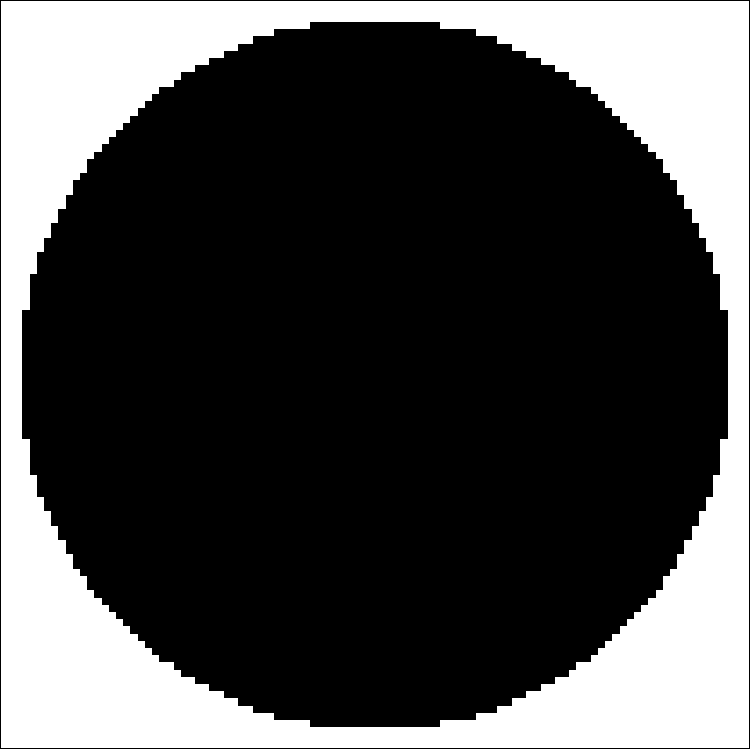
\includegraphics[ width = 1.5in ]{pdf/fourier/disk_bw_0100}\\
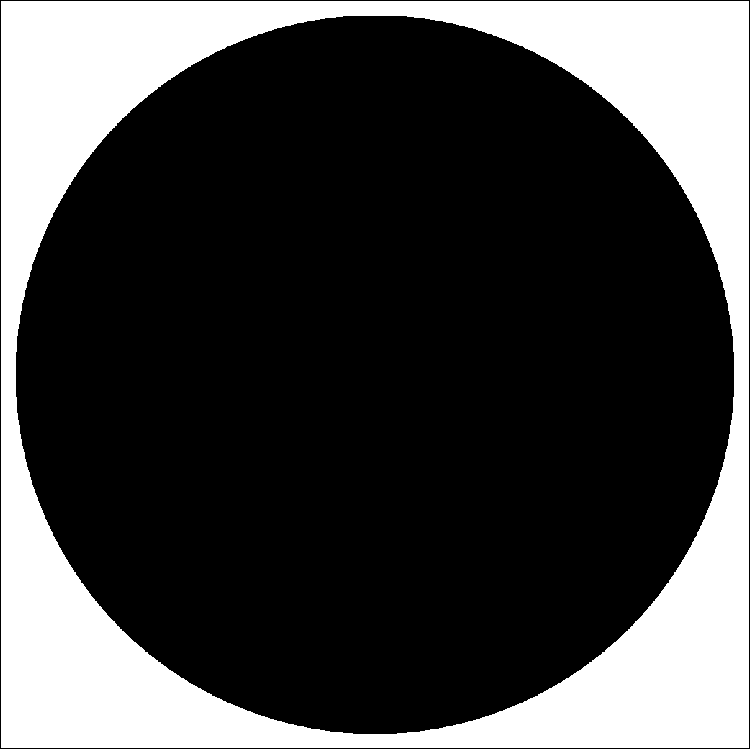
\includegraphics[ width = 1.5in ]{pdf/fourier/disk_bw_1000}\\

\end{tabular}
\end{center}
\label{tab:fourier:disk}
\caption{default}
\end{table}%
\section{The disk}

%%%
\subsection{Softened edges edges}
\begin{table}[htdp]
\begin{center}
\begin{tabular}{cc}


\includegraphics[ width = 1.5in ]{pdf/fourier/dither_0003}\\
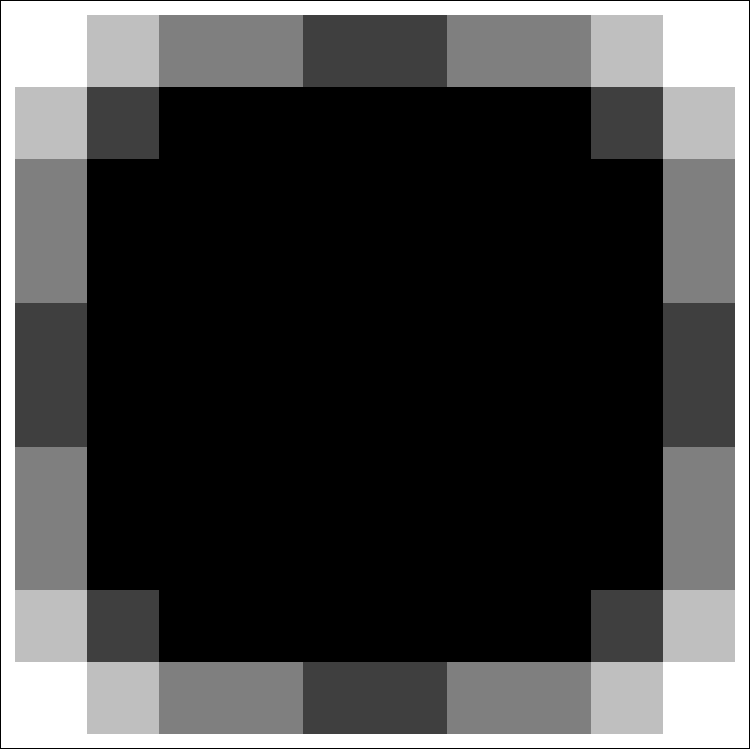
\includegraphics[ width = 1.5in ]{pdf/fourier/dither_0010}\\
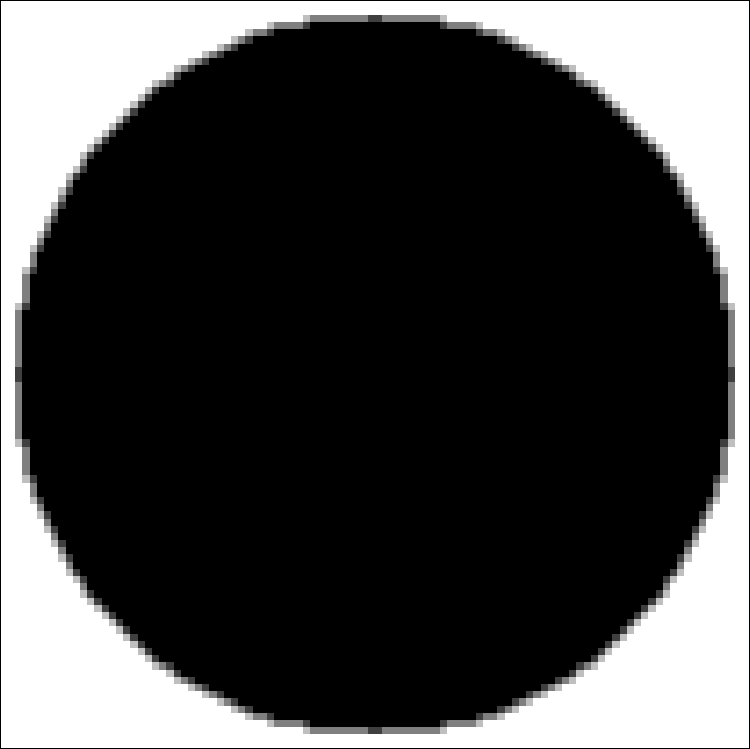
\includegraphics[ width = 1.5in ]{pdf/fourier/dither_00100}\\
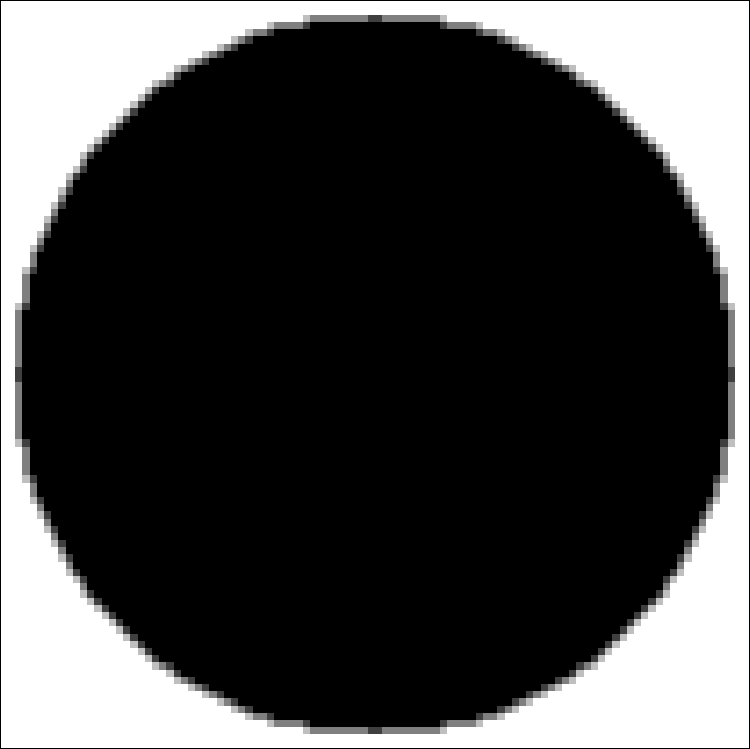
\includegraphics[ width = 1.5in ]{pdf/fourier/dither_00100}\\

\end{tabular}
\end{center}
\label{tab:fourier:dither}
\caption{default}
\end{table}%

\endinput
\renewcommand{\object}{diamond}
\renewcommand{\where} {\base\object/}    %%%%%%%%%%%%%%%%%
\begin{table}[htdp]
\begin{center}
\begin{tabular}{ccccc}
	\titlea \\
	\grafa{\where A__0003} &&
	\grafa{\where Y__0003} &
	\grafa{\where S__0003} &
	\grafa{\where Xt_0003} \\[5pt]
    %%%
	\grafa{\where A__0005} &&
	\grafa{\where Y__0005} &
	\grafa{\where S__0005} &
	\grafa{\where Xt_0005} \\[5pt]
    %%%
	\grafa{\where A__0010} &&
	\grafa{\where Y__0010} &
	\grafa{\where S__0010} &
	\grafa{\where Xt_0010} \\[5pt]
    %%%
	\grafa{\where A__0025} &&
	\grafa{\where Y__0025} &
	\grafa{\where S__0025} &
	\grafa{\where Xt_0025} \\[5pt]
    %%%
	\grafa{\where A__0050} &&
	\grafa{\where Y__0050} &
	\grafa{\where S__0050} &
	\grafa{\where Xt_0050} \\[5pt]
    %%%
	\grafa{\where A__0100} &&
	\grafa{\where Y__0100} &
	\grafa{\where S__0100} &
	\grafa{\where Xt_0100} \\[5pt]
%%%
\end{tabular}
\end{center}
\label{tab:8:diamond}
\caption[The \svdl \ for the \object]{The \svdl \ for the \object. The matrices are square and have dimensions \ncases.}
\end{table}%


\endinput
%% full rank
\renewcommand{\object}{Toeplitz}          %%%%%%%%%%%%%%%%%
\renewcommand{\where} {\base\object/}    %%%%%%%%%%%%%%%%%
\begin{table}[htdp]
\begin{center}
\begin{tabular}{ccccc}
	\titlea \\
	\grafa{\where A__0003} &&
	\grafa{\where Y__0003} &
	\grafa{\where S__0003} &
	\grafa{\where Xt_0003} \\[5pt]
    %%%
	\grafa{\where A__0005} &&
	\grafa{\where Y__0005} &
	\grafa{\where S__0005} &
	\grafa{\where Xt_0005} \\[5pt]
    %%%
	\grafa{\where A__0010} &&
	\grafa{\where Y__0010} &
	\grafa{\where S__0010} &
	\grafa{\where Xt_0010} \\[5pt]
    %%%
	\grafa{\where A__0025} &&
	\grafa{\where Y__0025} &
	\grafa{\where S__0025} &
	\grafa{\where Xt_0025} \\[5pt]
    %%%
	\grafa{\where A__0050} &&
	\grafa{\where Y__0050} &
	\grafa{\where S__0050} &
	\grafa{\where Xt_0050} \\[5pt]
    %%%
	\grafa{\where A__0100} &&
	\grafa{\where Y__0100} &
	\grafa{\where S__0100} &
	\grafa{\where Xt_0100} \\[5pt]
%%%
\end{tabular}
\end{center}
\label{tab:8:Toeplitz}
\caption[The \svdl \ for the \object]{The \svdl \ for the \object. The matrices are square and have dimensions \ncases.}
\end{table}%

\endinput
\renewcommand{\object}{Hankel}           %%%%%%%%%%%%%%%%%
\renewcommand{\where} {\base\object/}    %%%%%%%%%%%%%%%%%
\begin{table}[htdp]
\begin{center}
\begin{tabular}{ccccc}
	\titlea \\
	\grafa{\where A__0003} &&
	\grafa{\where Y__0003} &
	\grafa{\where S__0003} &
	\grafa{\where Xt_0003} \\[5pt]
    %%%
	\grafa{\where A__0005} &&
	\grafa{\where Y__0005} &
	\grafa{\where S__0005} &
	\grafa{\where Xt_0005} \\[5pt]
    %%%
	\grafa{\where A__0010} &&
	\grafa{\where Y__0010} &
	\grafa{\where S__0010} &
	\grafa{\where Xt_0010} \\[5pt]
    %%%
	\grafa{\where A__0025} &&
	\grafa{\where Y__0025} &
	\grafa{\where S__0025} &
	\grafa{\where Xt_0025} \\[5pt]
    %%%
	\grafa{\where A__0050} &&
	\grafa{\where Y__0050} &
	\grafa{\where S__0050} &
	\grafa{\where Xt_0050} \\[5pt]
    %%%
	\grafa{\where A__0100} &&
	\grafa{\where Y__0100} &
	\grafa{\where S__0100} &
	\grafa{\where Xt_0100} \\[5pt]
%%%
\end{tabular}
\end{center}
\label{tab:8:Hankel}
\caption[The \svdl \ for the \object]{The \svdl \ for the \object. The matrices are square and have dimensions \ncases.}
\end{table}%

\endinput
\renewcommand{\object}{ramp}                    %%%%%%%%%%%%%%%%%
\renewcommand{\where} {\base\object/}    %%%%%%%%%%%%%%%%%
\begin{table}[htdp]
\begin{center}
\begin{tabular}{ccccc}
	\titlea \\
	\grafa{\where A__0003} &&
	\grafa{\where Y__0003} &
	\grafa{\where S__0003} &
	\grafa{\where Xt_0003} \\[5pt]
    %%%
	\grafa{\where A__0005} &&
	\grafa{\where Y__0005} &
	\grafa{\where S__0005} &
	\grafa{\where Xt_0005} \\[5pt]
    %%%
	\grafa{\where A__0010} &&
	\grafa{\where Y__0010} &
	\grafa{\where S__0010} &
	\grafa{\where Xt_0010} \\[5pt]
    %%%
	\grafa{\where A__0025} &&
	\grafa{\where Y__0025} &
	\grafa{\where S__0025} &
	\grafa{\where Xt_0025} \\[5pt]
    %%%
	\grafa{\where A__0050} &&
	\grafa{\where Y__0050} &
	\grafa{\where S__0050} &
	\grafa{\where Xt_0050} \\[5pt]
    %%%
	\grafa{\where A__0100} &&
	\grafa{\where Y__0100} &
	\grafa{\where S__0100} &
	\grafa{\where Xt_0100} \\[5pt]
%%%
\end{tabular}
\end{center}
\label{tab:8:ramp}
\caption[The \svdl \ for the \object]{The \svdl \ for the \object. The matrices are square and have dimensions \ncases.}
\end{table}%


\endinput
\renewcommand{\object}{tones}                   %%%%%%%%%%%%%%%%%
\renewcommand{\where} {\base\object/}    %%%%%%%%%%%%%%%%%
\begin{table}[htdp]
\begin{center}
\begin{tabular}{ccccc}
	\titlea \\
	\grafa{\where A__0003} &&
	\grafa{\where Y__0003} &
	\grafa{\where S__0003} &
	\grafa{\where Xt_0003} \\[5pt]
    %%%
	\grafa{\where A__0005} &&
	\grafa{\where Y__0005} &
	\grafa{\where S__0005} &
	\grafa{\where Xt_0005} \\[5pt]
    %%%
	\grafa{\where A__0010} &&
	\grafa{\where Y__0010} &
	\grafa{\where S__0010} &
	\grafa{\where Xt_0010} \\[5pt]
    %%%
	\grafa{\where A__0025} &&
	\grafa{\where Y__0025} &
	\grafa{\where S__0025} &
	\grafa{\where Xt_0025} \\[5pt]
    %%%
	\grafa{\where A__0050} &&
	\grafa{\where Y__0050} &
	\grafa{\where S__0050} &
	\grafa{\where Xt_0050} \\[5pt]
    %%%
	\grafa{\where A__0100} &&
	\grafa{\where Y__0100} &
	\grafa{\where S__0100} &
	\grafa{\where Xt_0100} \\[5pt]
%%%
\end{tabular}
\end{center}
\label{tab:8:tones}
\caption[The \svdl \ for the \object]{The \svdl \ for the \object. The matrices are square and have dimensions \ncases.}
\end{table}%

\endinput
\renewcommand{\object}{bones}            %%%%%%%%%%%%%%%%%
\renewcommand{\where} {\base\object/}    %%%%%%%%%%%%%%%%%
\begin{table}[htdp]
\begin{center}
\begin{tabular}{ccccc}
	\titlea \\
	\grafa{\where A__0003} &&
	\grafa{\where Y__0003} &
	\grafa{\where S__0003} &
	\grafa{\where Xt_0003} \\[5pt]
    %%%
	\grafa{\where A__0005} &&
	\grafa{\where Y__0005} &
	\grafa{\where S__0005} &
	\grafa{\where Xt_0005} \\[5pt]
    %%%
	\grafa{\where A__0010} &&
	\grafa{\where Y__0010} &
	\grafa{\where S__0010} &
	\grafa{\where Xt_0010} \\[5pt]
    %%%
	\grafa{\where A__0025} &&
	\grafa{\where Y__0025} &
	\grafa{\where S__0025} &
	\grafa{\where Xt_0025} \\[5pt]
    %%%
	\grafa{\where A__0050} &&
	\grafa{\where Y__0050} &
	\grafa{\where S__0050} &
	\grafa{\where Xt_0050} \\[5pt]
    %%%
	\grafa{\where A__0100} &&
	\grafa{\where Y__0100} &
	\grafa{\where S__0100} &
	\grafa{\where Xt_0100} \\[5pt]
%%%
\end{tabular}
\end{center}
\label{tab:8:bones}
\caption[The \svdl \ for the \object]{The \svdl \ for the \object. The matrices are square and have dimensions \ncases.}
\end{table}%

\endinput
\renewcommand{\object}{Hilbert}          %%%%%%%%%%%%%%%%%
\renewcommand{\where} {\base\object/}    %%%%%%%%%%%%%%%%%
\begin{table}[htdp]
\begin{center}
\begin{tabular}{ccccc}
	\titlea \\
	\grafa{\where A__0003} &&
	\grafa{\where Y__0003} &
	\grafa{\where S__0003} &
	\grafa{\where Xt_0003} \\[5pt]
    %%%
	\grafa{\where A__0005} &&
	\grafa{\where Y__0005} &
	\grafa{\where S__0005} &
	\grafa{\where Xt_0005} \\[5pt]
    %%%
	\grafa{\where A__0010} &&
	\grafa{\where Y__0010} &
	\grafa{\where S__0010} &
	\grafa{\where Xt_0010} \\[5pt]
    %%%
	\grafa{\where A__0015} &&
	\grafa{\where Y__0015} &
	\grafa{\where S__0015} &
	\grafa{\where Xt_0015} \\[5pt]
    %%%
	\grafa{\where A__0020} &&
	\grafa{\where Y__0020} &
	\grafa{\where S__0020} &
	\grafa{\where Xt_0020} \\[5pt]
    %%%
	\grafa{\where A__0050} &&
	\grafa{\where Y__0050} &
	\grafa{\where S__0050} &
	\grafa{\where Xt_0050} 
%%%
\end{tabular}
\end{center}
\label{tab:8:bones}
\caption[The \svdl \ for the \object]{The \svdl \ for the \object. The matrices are square and have dimensions \ncases.}
\end{table}%

\endinput
\renewcommand{\object}{random}          %%%%%%%%%%%%%%%%%
\renewcommand{\where} {\base\object/}    %%%%%%%%%%%%%%%%%
\begin{table}[htdp]
\begin{center}
\begin{tabular}{ccccc}
	\titlea \\
	\grafa{\where A__0003} &&
	\grafa{\where Y__0003} &
	\grafa{\where S__0003} &
	\grafa{\where Xt_0003} \\[5pt]
    %%%
	\grafa{\where A__0005} &&
	\grafa{\where Y__0005} &
	\grafa{\where S__0005} &
	\grafa{\where Xt_0005} \\[5pt]
    %%%
	\grafa{\where A__0010} &&
	\grafa{\where Y__0010} &
	\grafa{\where S__0010} &
	\grafa{\where Xt_0010} \\[5pt]
    %%%
	\grafa{\where A__0025} &&
	\grafa{\where Y__0025} &
	\grafa{\where S__0025} &
	\grafa{\where Xt_0025} \\[5pt]
    %%%
	\grafa{\where A__0050} &&
	\grafa{\where Y__0050} &
	\grafa{\where S__0050} &
	\grafa{\where Xt_0050} \\[5pt]
    %%%
	\grafa{\where A__0100} &&
	\grafa{\where Y__0100} &
	\grafa{\where S__0100} &
	\grafa{\where Xt_0100} \\[5pt]
%%%
\end{tabular}
\end{center}
\label{tab:8:random}
\caption[The \svdl \ for the \object]{The \svdl \ for the \object. The matrices are square and have dimensions \ncases.}
\end{table}%

\endinput
%% full rank
\input{chapters/"ch 09"/"tables/Zernike 00"}

\endinput